\chapter{Résultats \& discussions}\label{chap:result_discussions}
\chaptermark{Résultats & discussions}
%\minitoc
  
L'application pratique de tout modèle conceptuel est la pierre de touche qui révèle sa validité et sa pertinence. Dans ce chapitre consacré aux résultats, les conclusions tirées de la mise en pratique des concepts discutés précédemment sont présentées. Nous réexaminons d'abord la valeur de la connaissance, en se concentrant spécifiquement sur l'utilisation de l'entropie comme métrique de la qualité de la connaissance (\ref{subsubsec:res_entropie}). Les implications et les observations découlant de cette approche seront présentées en détail. Ensuite, les résultats relatifs au calcul des contributions (\ref{subsec:res_calcul des contributions}) sont exposés, révélant comment ces méthodes se traduisent dans des situations concrètes et quelle valeur elles apportent à l'ensemble de l'écosystème.

Une fois les résultats exposés, un examen détaillé des aspects centraux du modèle d'intéressement financier est entrepris. La valeur de la connaissance (\ref{subsec: discuss_kg_value}), étant une pierre angulaire, est revisitée pour discuter des implications, des nuances, et des éventuels ajustements requis. De même, le calcul des contributions est scruté à la loupe, invitant à une réflexion sur sa pertinence, ses limites et ses améliorations potentielles (\ref{subsec: discuss_contrib}). Enfin, une exploration de la complexité de la solution s'ensuit, évaluant sa pertinence pour une mise en œuvre sur une blockchain, mettant en lumière les enjeux techniques et conceptuels à relever (voir la section \ref{sec:discuss_complexity}). Ce chapitre vise à offrir une perspective équilibrée, en soulignant à la fois les apports du modèle et les domaines nécessitant une attention supplémentaire.

\begin{comment}
Ce chapitre vise à mettre en lumière les forces et les potentialités du modèle d'intéressement financier et à offrir des insights sur sa mise en œuvre effective.
\end{comment}

\section{Résultats} \label{sec: resultats}


\subsection{Valeur de la connaissance} \label{subsec:res_kg_value}

\subsubsection{Utilisation de l'entropie comme métrique de qualité de la connaissance} \label{subsubsec:res_entropie}
L'hypothèse de base en utilisant l'entropie pour évaluer la qualité de la connaissance est de pouvoir quantifier objectivement la dispersion des valeurs dans les données et d'identifier les tendances de regroupement. Afin d'évaluer cette hypothèse, des échantillons de diverses tailles ont été générés en suivant trois distributions de probabilité : normale, uniforme et exponentielle. Les échantillons ont été obtenus en faisant varier les paramètres de ces différentes lois comme consignés dans les tableaux \ref{table:xp_normale}, \ref{table:xp_exponentelle} et \ref{table:xp_uniforme} : 


\begin{table}[h]
\centering
\begin{tabular}{l c}
\toprule
Paramètres & Valeurs  \\
\midrule
taille & 15, 30, 60, 120, 240, 480, 960, 1920, 4000, 6000, 8000, 10000 \\
$\mu$ & 0 \\
$\sigma$ & 0.1, 0.2, 0.3, 0.4, 0.5, 0.6, 0.7, 0.8, 0.9, 1.0 \\
\bottomrule
\end{tabular}
\caption{Valeurs prise par les paramètres pour générer les échantillons normalement distribués } \label{table:xp_normale}
\end{table}


\begin{table}[h]
\centering
\begin{tabular}{l c}
\toprule
Paramètres & Valeurs  \\
\midrule
taille & 15, 30, 60, 120, 240, 480, 960, 1920, 4000, 6000, 8000, 10000 \\
$\lambda$ & $1, \frac{1}{\sqrt{2}}, \frac{1}{\sqrt{3}}, \frac{1}{\sqrt{4}}, \frac{1}{\sqrt{5}}, \frac{1}{\sqrt{6}}, \frac{1}{\sqrt{7}}, \frac{1}{\sqrt{8}}, \frac{1}{\sqrt{9}}, \frac{1}{\sqrt{10}}$ \\
\bottomrule
\end{tabular}
\caption{Valeurs prise par les paramètres pour générer les échantillons de loi de distribution exponentielle } \label{table:xp_exponentelle}
\end{table}


\begin{table}[h]
\centering
\begin{tabular}{l c}
\toprule
Paramètres & Valeurs  \\
\midrule
taille & 15, 30, 60, 120, 240, 480, 960, 1920, 4000, 6000, 8000, 10000 \\
Centre & 0\\
r & 0.1, 0.2, 0.3, 0.4, 0.5, 0.6, 0.7, 0.8, 0.9, 1.0 \\
a = Centre - r & b = Centre + r \\
\bottomrule
\end{tabular}
\caption{Valeurs prise par les paramètres pour générer les échantillons de loi de uniforme } \label{table:xp_uniforme}
\end{table}

De plus, différentes méthodes pour discrétiser les données ont été évaluées, esentiellement de celles disponibles dans la librairie Python NumPy (\cite{harris_array_2020}) pour le calcul des classes d'histogrammes. Les méthodes utilisées pour le calcul du nombre de classes sont la méthode <<racine carrée>>, la méthode <<auto>> et la méthode <<Doane>>. La méthode racine carré consiste à utiliser un nombre de classes égal à la racine carré du nombre d'échantillons. La méthode auto choisit automatiquement entre une méthode dite <<FD>> et une de <<Sturge>>. Enfin la méthode <<Doane>> calcule le nombre de classe en prenant en compte la dispersion dans les données.

Pour chaque échantillon généré, l'entropie a été calculée en utilisant chaque méthode respective, et les résultats sont présentés dans la figure \ref{fig:res_entropie}.

\begin{figure}[h]
    \centering
    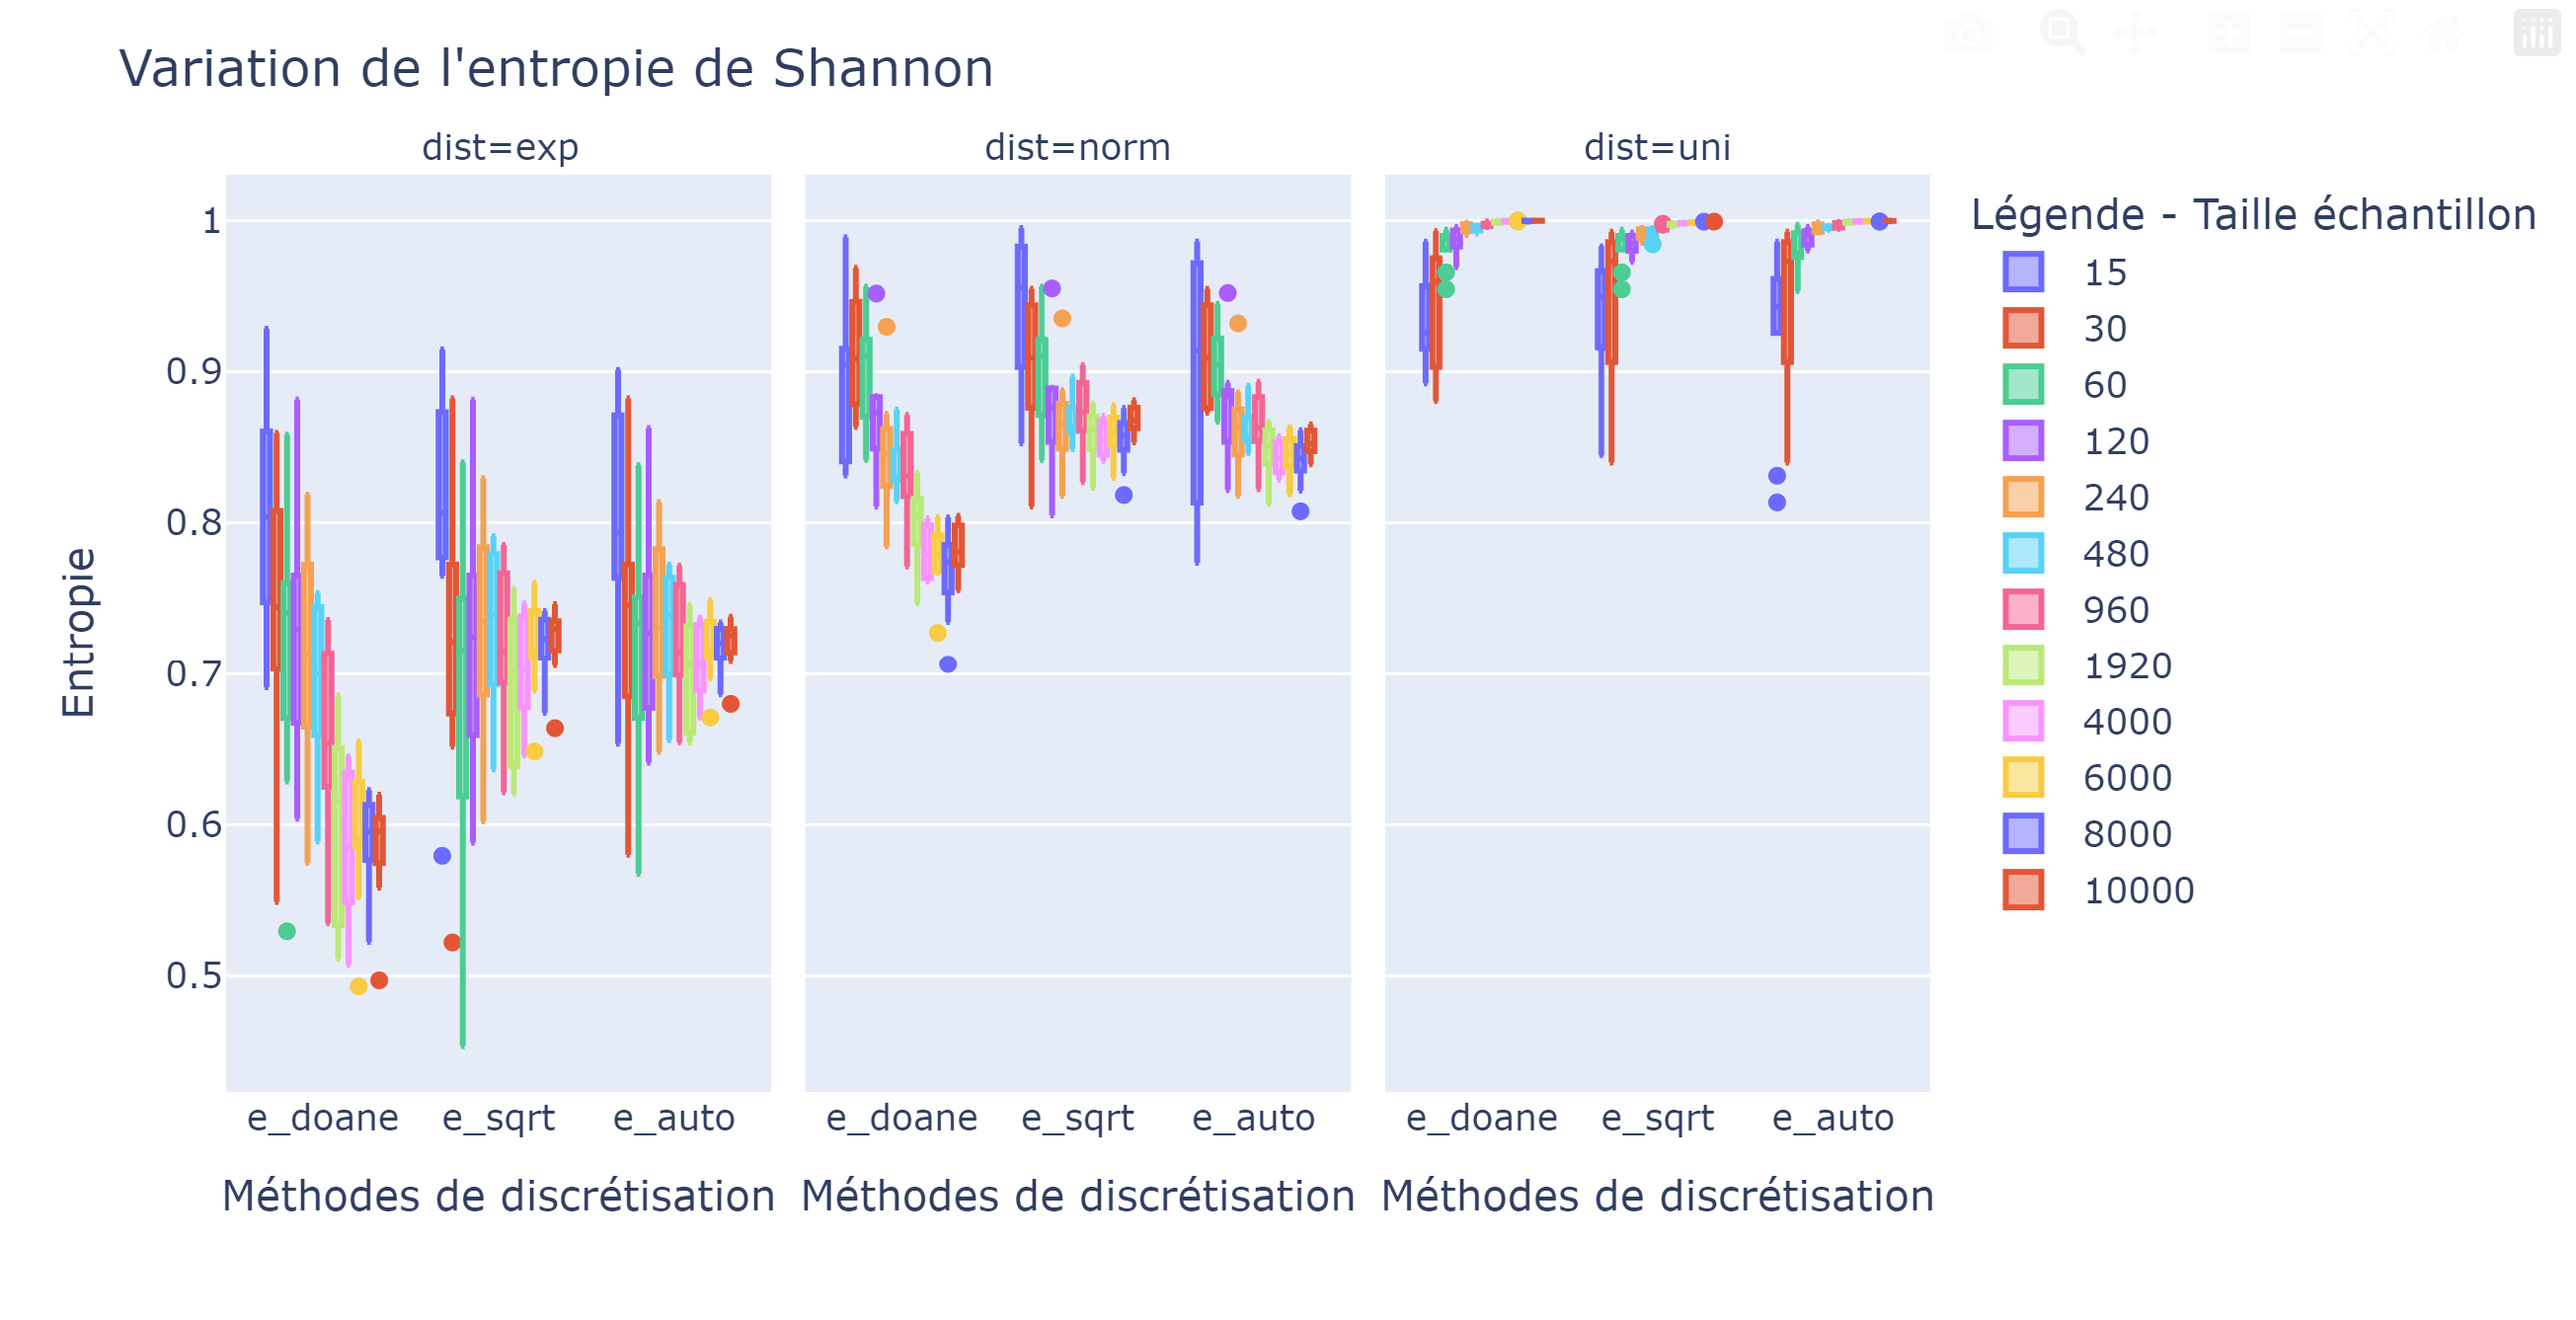
\includegraphics[width=0.8\textwidth]{ILLUSTRATIONS/entropie_size_box_distxp.png}
    \caption{Evolution de l'entropie en fonction de la distribution sous-jacente et de la méthode de calcul}
    \label{fig:res_entropie}
\end{figure}


En évaluant les résultats présentés sur la figure \ref{fig:res_entropie}, une conclusion émerge de manière naturelle, indiquant que l'entropie est une métrique pertinente pour distinguer les distributions qui peuvent être présentes dans les données. 

En observant les niveaux d'entropie, une tendance cohérente se dégage : l'entropie de la distribution uniforme est toujours supérieure à celle de la distribution normale, qui à son tour est plus élevée que celle de la distribution exponentielle. Cette hiérarchie découle naturellement des caractéristiques intrinsèques de chaque distribution. La distribution uniforme, avec son égalité de probabilité, présente une incertitude maximale et donc une entropie maximale. La distribution normale, bien qu'elle puisse être plus concentrée, reste moins prévisible qu'une distribution exponentielle, qui décroît rapidement. Cette relation entre les niveaux d'entropie offre une métrique pertinente pour distinguer les différentes distributions présentes dans les données.

En examinant la distribution uniforme, on constate que l'entropie converge systématiquement vers 1, quelle que soit la méthode de discrétisation. Cela est en adéquation avec l'idée que chaque valeur a une probabilité égale d'apparaître, conduisant à une situation d'incertitude maximale et d'entropie totale. Cette convergence uniforme souligne que toutes les méthodes de discrétisation parviennent à capturer la nature fondamentale de la distribution uniforme.

Cependant, des distinctions significatives sont observées pour les distributions normale et exponentielle. Les méthodes <<auto>> et <<sqrt>> produisent des valeurs d'entropie plus élevées que la méthode <<Doane>> \footnote{<<sqrt>> pour racine carrée}. Il est possible que les nombres de classes produits par les méthodes <<auto>> et <<sqrt>>, relativement grands par rapport à celui produit par la méthode <<Doane>>, aient pour conséquence de répartir les effectifs de manière plus équilibrée entre les classes. Cette répartition peut donner l'impression d'une distribution plus uniforme et pourrait effectivement augmenter l'entropie, car il y aurait moins de classes dominantes. C'est la raison pour laquelle il est pertinent d'opter pour la méthode de <<Doane>>, qui prend en considération l'asymétrie (\textit{skew}) des distributions. Contrairement à d'autres méthodes qui pourraient surévaluer l'entropie en générant un grand nombre de classes, la méthode <<Doane>> ajuste le nombre de classes en fonction de la \textit{skweness} des données. Cela prévient une fragmentation excessive qui pourrait altérer la représentation fidèle de la distribution et potentiellement exagérer l'entropie.


\subsection{Calcul des contributions} \label{subsec:res_calcul des contributions}

Dans cette section, les résultats d'un test pour le calcul des contributions en utilisant la valeur de Shapley sont exposés. Le test a consisté à générer un tableau de données, qui fait office de connaissance, à l'aide du code \ref{code:data_gen} (\autoref{ansec:autres}) ; Pour simplifier, chaque colonne a été considérée comme une donnée individuelle ayant contribué à la création de cette connaissance. Le tableau généré a ensuite été utilisé comme entrée du code \ref{ansec:shapley_compute} qui est la traduction en python de l'algorithme \ref{algo:shapley_approx}. Les résultats sont consignés dans le tableau \ref{table:result_shapley}.

\begin{table}[h]
\centering
\begin{tabular}{l c c c c}
\toprule
Données & Data 1 & Data 2 & Data 3 & Entropie $K_G$  \\
\midrule
Valeur de Shapley & 0.00315 & -0.02862 & 0.02552 & 0.87722 \\
\bottomrule
\end{tabular}
\caption{Résultats du calcul de la valeur de shapley sur une donnée} \label{table:result_shapley}
\end{table}

Il est possible d'observer des valeurs de Shapley positives pour "Data 1" et "Data 3" alors que la valeur de Shapley pour "Data 2" est négative. Cela peut s'expliquer par le fait que la valeur de Shapley est définie pour permettre le partage équitable de fonctions de valeur transférables et superaditives. Cependant, dans le contexte de cette étude, l'entropie calculée pour une connaissance ne suit pas cette propriété. Sinon, la somme des valeurs de Shapley de chaque donnée aurait approximativement abouti à 0,87722.  

Par ailleurs, la valeur de Shapley calculant la contribution moyenne d'un joueur au sein d'une coalition à la fonction de valeur, une valeur de Shapley négative pourrait dire que la donnée en question a pour effet moyen de réduire l'entropie moyenne de la connaissance alors qu'une valeur de Shapley positive aurait pour effet moyen de l'augmenter. Alors, il serait possible d'établir un classement du plus contributif au moins contributif. A partir de ces valeurs de Shapley il est possible d'appliquer des transformations qui conservent cette relations d'ordre pour le calcul d'un poids qui ferait office de contribution. 

De toute évidence la valeur de Shapley ne semble pas répondre à la question du calcul équitable des contributions.

\subsection{Complexité de la marketplace} \label{subsec:res_complexity}

Au sein de cette section, la complexité inhérente aux codes de la marketplace (Annexe \ref{annexe:codes_python}) est exposée. Cette démarche permet de mieux appréhender les éventuels coûts associés à leur exécution. Pour ce faire, la notation asymptotique, également connue sous le nom de notation de Bachmann-Landau, est employée. Cette notation offre un cadre pour évaluer comment les performances pourraient évoluer en fonction de la taille des données d'entrée. Le tableau \ref{table:notations_asymptotiques} synthétise les complexités temporelles et spatiales du code de la marketplace, exprimées en notations asymptotiques \footnote{La complexité temporelle d'un algorithme mesure le temps d'exécution en fonction de la taille de ses données d'entrée. La complexité spatiale, quant à elle, évalue l'utilisation de la mémoire pendant l'exécution de l'algorithme. La notation \textbf{$O$}, ou notation asymptotique, est un outil fondamental pour décrire ces complexités.  Par exemple, une complexité temporelle en $O(n^2)$ signifie que le temps d'exécution croît quadratiquement avec la taille $n$ des données.}.


\begin{table}[h]
\centering
\begin{tabular}{c c c c c}
\toprule
Référence & Fonction & Complexité temporelle & Complexité spatiale\\
\bottomrule
\ref{ansec:alloc_compute}& Fonction d'allocation & $O(l^2 \log(l) \cdot v)$
 & $O(l \cdot v)$\\
 \midrule
 \ref{ansec:shannon_compute}& Calcul de l'entropie & $O(l^2 \cdot v)$
 & $O(l)$\\
  \midrule
 \ref{ansec:shapley_compute}& Calcul des valeurs de Shapley & $O(K \cdot N_k \cdot l \cdot v)$
 & $O(l \cdot v)$\\
  \midrule
 \ref{ansec:vkg_compute}& Valeur de la connaissance & $O(l \cdot v + u)$
 & $O(1)$\\
  \midrule
 \ref{ansec:priceupdate_compute}& Mise à jour du prix de reserve& $O(|B_{net}(\epsilon)|)$
 & $O(|B_{net}(\epsilon)|)$\\
\bottomrule
\end{tabular}
\caption{complexités temporelles et spatiales en notations asymptotiques} \label{table:notations_asymptotiques}
\end{table}

$l$ et $v$ désignent respectivement le nombre de lignes et de colonnes de la connaissance $K_{G_k}$, $K$ le nombre d'échantillon pour approcher la valeur de Shapley pour une donnée $D_{k,j}$ de $D_k$, $N_k$ le nombre de données de $D_k$, $|B_{net}(\epsilon)|$ le nombre de prix experts utilisées par la marketplace, et $u$ le nombre d'itérations pour l'intégration numérique dans le calcul de la valeur de la connaissance . 

Une analyse préliminaire du tableau \ref{table:notations_asymptotiques} permet de voir que l'ensemble des fonctions de la marketplace à une complexité en $O(f(l,v))$, sauf a fonction de mise à jour du prix de réserve qui s'exécute en temps linéaire avec la taille de la collection des prix experts mais fait appel en boucle à la fonction de calcul de la valeur de la connaissance (algorithme \ref{algo:price_update}). En d'autres termes, la coût d'exécution de la marketplace est fortement lié à la taille de la connaissance qui fait l'objet de la transaction.

Ensuite, sur le même tableau il est possible d'observer que l'ensemble des fonctions de la marketplace s'exécutent au plus en temps polynomiale quand la taille des entrée devient très grand. Cette caractéristique présente un intérêt fondamental dans le domaine de la complexité algorithmique et de l'efficacité computationnelle. Lorsqu'une fonction ou un algorithme s'exécute en temps polynomial par rapport à la taille des données d'entrée, cela signifie que le temps d'exécution croît de manière raisonnable et prévisible à mesure que les données augmentent.


\section{Discussions} \label{sec:discussions}

\subsection{Valeur de la connaissance} \label{subsec: discuss_kg_value}

Les résultats présentés dans la section \ref{subsec:res_kg_value} montrent que l'entropie peut être une métrique efficace pour évaluer la valeur de la connaissance dans les ensembles de données. Cette mesure reflète la diversité et la complexité des données, permettant ainsi d'estimer leur pertinence. Cependant, les résultats de cette étude mettent en évidence que la méthode de discrétisation de l'entropie peut avoir un impact significatif sur les valeurs d'entropie obtenues. Ce constat  souligne l'importance de choisir judicieusement la méthode de discrétisation pour éviter des évaluations erronées.

On peut retrouver l'usage de l'entropie de Shannon dans des fonctions de prix de données avec \citeauthor{deep_qirana_2017} (\citeyear{deep_qirana_2017}). La présente étude est différente en deux points : Premièrement \citeauthor{deep_qirana_2017} s'intéressent à la tarification des requêtes sur une base de donnée alors que cette étude s'intéresse à la tarification d'une connaissance dans son entièreté ; Deuxièmement \citeauthor{deep_qirana_2017} suppose que la base de données a un prix connu et le prix de chaque requête est non-nul et d'autant plus grand si l'information qu'elle apporte est nouvelle par rapport aux requêtes précédentes \footnote{le prix de la requêtes est donnée par l'entropie de Shannon directement. Notre avis est que, étant donnée que cette entropie est calculée sur des symboles qui sont des hashs des requêtes, la moindre décimale de différence dans les résultats d'une requête produit une nouvelle valeur de hash. Cela aura pour conséquence une entropie toujours maximale avec des prix toujours croissants à mesure que la taille des requêtes augmente car intuitivement la probabilité d'un tout nouveau hash est grande.} ; Cette étude adresse plutôt une situation où le fournisseur de données ne sait pas donner de prix à son bien et souhaite en tirer le maximum pour chaque nouveau consommateur, et utilise l'entropie couplée à une fonction de modification de la connaissance comme fonction d'allocation dans un système d'enchère optimal au sens de \citeauthor{myerson_optimal_1981}(\citeyear{myerson_optimal_1981}). Cependant, les deux approches montrent comment l'entropie peut être utilisée comme un outil puissant pour quantifier des caractéristiques complexes des données.

Cette étude a montré l'intérêt d'utiliser l'entropie de Shannon pour évaluer la valeur d'une donnée, d'une connaissance. Toutefois, les constructions faites concernent essentiellement des données sous format tabulaire à taille fixe, ce qui ne couvre pas la diversité des sources et des formats de données disponibles. L'extension des résultats de cette étude à d'autres formes de données n'est pas non plus examinée. De plus, l'impact de ces méthodes de discrétisation sur les distributions multimodales n'a pas été étudié. Par ailleurs, les considérations relatives à l'entropie pour les données de type catégorielles ne sont pas abordées dans cette étude, bien que des similitudes puissent être observées étant donné que la discrétisation implique la création de catégories.

%Dans la section \ref{subsec:alteration_func} 

La fonction d'altération présentée en \ref{subsubsec:kg_value} traite les colonnes les unes après les autres. La cohérence du résultat de cette fonction n'est pas garantie, étant donné que ce ne sont pas nécessairement les mêmes lignes qui seront modifiées dans chaque colonne de la connaissance.

Pour terminer, il est à noter que, comme bon nombre d'études abordant des problématiques similaires, celle-ci demeure principalement théorique et n'a pas été mise en œuvre concrètement. Une étape suivante pourrait consister à concrétiser ce système dans un cadre d'utilisation, même si cette mise en œuvre ne se réalise pas nécessairement au sein des nœuds d'une blockchain.


\subsection{Calcul des contributions} \label{subsec: discuss_contrib}


Les résultats presentés dans la section \ref{subsec:res_calcul des contributions} montrent que dans les conditions de cette étude, la valeur de Shapley ne permet pas une allocation équitable des ressources. En effet, dans des situations où la fonction de valeur (l'entropie dans cette étude) n'est pas superaditive, les conditions pour l'application de la valeur de Shapley ne sont pas atteintes ayant pour conséquences des contributions aberrantes soulignant ainsi les limites de la valeur de Shapley dans ces contextes spécifiques.

Cette absence de réponses définitives quant au calcul des contributions dans les jeux collaboratifs où la fonction de valeur est une grandeur non additive, ouvre la voie à des investigations plus approfondies visant à élucider des méthodes de calcul des contributions dans des contextes similaires à celle de cette étude. Des études sur la question émerge déjà avec \cite{khan_incentive_2023} qui obtient les mêmes type de résultats que ceux présentés dans cette étude avec la valeur de Shapley qu'elle compare à une allocation de ressources par la résolution d'un problème de faillite avec la méthode du Talmud. Cette convergence souligne l'importance des conclusions de cette étude et leur pertinence dans un contexte plus large.

En outre, plutôt que de se focaliser sur la répartition de la valeur issue de la connaissance, il serait envisageable d'implémenter directement le système d'enchères exposé dans cette étude en relation avec les données, tout en demeurant dans le contexte de l'économie de la connaissance. La distinction réside dans le fait que les enchères seraient utilisées pour obtenir temporairement le droit d'utiliser les données au sein d'un service de traitement, dans le but de créer de la connaissance, toujours au sein de l'écosystème OKP4.


\subsection{Complexité de la solution et adéquation pour une implémentation sur une Blockchain} \label{sec:discuss_complexity}

Comme présenté dans la section \ref{subsec:res_complexity} les fonctions de la marketplace devraient pouvoir s'exécuter en temps polynomiale avec la taille de leurs données d'entrée. Toutefois, cela est à mettre en perspective du type de données d'entrée dont il s'agit : des tableaux de données. Il convient de rappeler que la plupart de ces fonctions présentent une complexité en $O(f(l,v))$. Dans un contexte de big data, exécuter ces fonctions sur des noeuds d'une blockchain est impraticable pour les raisons abordées en \ref{subsubsec:complex}. 

Par conséquent, il est de plus en plus évident qu'une automatisation du modèle d'intéressement via une blockchain pourrait ne plus être une voie viable. Néanmoins, une piste prometteuse peut être une mise en œuvre au sein d'un service du \textit{dataverse} en capitalisant sur les résultats issus de cette étude comme un point de départ dynamique. En effet, dans sa conception qui permet \textit{anything as a service} le protocole OKP4 peut externaliser ce type de calculs coûteux sur des infrastructures adéquates.

Dans la section \ref{subsec:model_pb} il a été introduit le \textit{knowledge graphe}. L'une des raisons à celà était d'étudier la dynamique de la répartition de la valeur le long de la généalogie d'une connaissance et le coût en espace de stocker les informations de ce graphe. Pour ce faire, il aurait fallu avoir des résultats probant avec la méthode de calcul des contribution exposée dans ce mémoire. Mais cette question semble ne plus se poser dans la mesure où la capacité d'une blockchain à exécuter les calculs à une génération de ce graphe est compromise. 


\begin{comment}

Nos résultats ont mis en évidence un défi majeur : les méthodes développées dans cette étude ont un coût d'exécution significativement élevé. Cette complexité computationnelle peut restreindre leur applicabilité dans des environnements où les ressources sont limitées, tels que les blockchains avec des contraintes de puissance de calcul et de stockage.

Une piste intéressante pour surmonter la contrainte de ressources serait d'envisager une implémentation hors de la blockchain, dans un environnement plus puissant. En utilisant des infrastructures informatiques plus robustes et flexibles, nous pourrions réduire le temps de calcul et permettre une évaluation plus rapide et efficace de la valeur de la connaissance.


- la valeur de shapley ne permet pas une allocation équitables dans les conditions de notre études.
- cette étude reste sans réponses quant au calcul des contribution.
- ses résultats coincident avec Afsana Khan
- Pour les piste de recherche serait de vérifier l'adéation de leur modèle avec notre contexte pour une grandeur non additive

ouverture : Afsana Khan parvient à des conclusion similaires pour la valeur de shapley, préconise l'utilisation de la méthode du talmud pour la résolution.


Dans cette section, nous aborderons en profondeur les principaux constats de notre étude concernant l'utilisation de la valeur de Shapley et ses implications pour l'allocation équitable des ressources. Nous discuterons également des découvertes qui restent en suspens, leurs parallèles avec d'autres travaux, et évoquerons des pistes de recherche futures pour poursuivre l'exploration de ces questions.

Dans cette section, nous examinerons en détail les principaux résultats de notre étude sur l'utilisation de l'entropie comme métrique pour évaluer la valeur de la connaissance et les implications pratiques de nos conclusions. Nous aborderons également les limitations de notre approche et les voies potentielles pour des recherches futures.

- Les méthodes développées dans cette étude ont un coût d'éxécution trop important
- Une piste serait d'envisager une implémentation hors de la blockchain dans un environnement plus puissant
- Défintivemnt


Dans cette étude nous avons introduit un système d'enchère entre des consommateurs de connaissance successifs, et l'algoritme de mise à jour du prix de réserve. Ce algorithme prend en entrée une liste de prix experts qui vont servir de prix de réserve sucessifs selon la dynamique de la marketplace. Cependant nous n'avons pas presenté comment choisir ces prix experts. 

De plus, nous avons constaté que le calcul de la valeur de la connaissance en utilisant l'équation de Myerson peut être coûteux en termes de ressources de calcul. Cette contrainte doit être prise en compte lors de l'application de cette approche dans des contextes réels.

Sous des contraintes de ressources de calcul suffisantes, notre étude suggère que l'entropie peut servir d'échelle pour fixer le prix d'une donnée comparativement à une autre. Cette interprétation offre un moyen concret d'appliquer nos résultats dans des scénarios de tarification de données, en prenant en compte leur diversité et leur complexité.

Malgré nos résultats prometteurs, notre étude présente certaines limitations. Tout d'abord, le temps de calcul de la solution proposée peut être un facteur limitant dans des applications en temps réel. De plus, nous reconnaissons que notre étude ne couvre pas la diversité complète des types de données disponibles, ce qui pourrait influencer l'applicabilité de nos résultats. Nous n'avons pas non plus testé notre méthode sur des distributions multimodales, ce qui pourrait révéler des nuances supplémentaires dans l'évaluation de la valeur de la connaissance.

De manière cruciale, si un ensemble de données traite de durées de vie avec une distribution exponentielle, il pourrait être sous-évalué en raison des limites de la façon dont l'entropie capture la diversité dans les données.

Enfin, le choix de modéliser la connaissance comme une jointure et de calculer une entropie moyenne suppose que nous devrions peut-être envisager de calculer la valeur d'une donnée plutôt que la valeur d'une connaissance. Cette perspective n'est en rien antagoniste à l'économie de la connaissance.

En conclusion, notre étude apporte une contribution significative à la compréhension de l'utilisation de l'entropie comme métrique pour évaluer la valeur de la connaissance. Les implications pratiques de nos résultats ouvrent la voie à des applications concrètes dans la tarification et la gestion des données. Cependant, il est impératif de prendre en compte les limitations identifiées et de poursuivre la recherche dans ces domaines pour affiner et généraliser nos conclusions.
\end{comment}


\begin{comment}
- récapitulatif des résultats :
L'entropie peut servir comme métrique de qualité pour l'évaluation de la valeur de la connaissance
La méthode de discrétisation de l'entropie peut influencer les valeurs d'entropie
Le calcul de la valeur de la connaissance en utilisant l'équation de Myerson est couteuse en ressources de calcul

- Comparaison avec la littérature :
Comparaison avec l'étude qui utilise d'entropie sur des hash de lignes pour évaluer des similitudes dans les données étant donnée un prix de base défini par le vendeur de données.

- interpretation pratiques : Sous contraintes de ressources de calciul suffisantes, l'entropie peut servir d'echelle pour fixer le prix d'une donnée comparativement à une autre.

-Limites : 
- le temps de calcul de la solution proposé
- Notre étude ne couvre pas la diversité des données disponibles
- Nous n'avons pas fait de test pour des distributions multimodales
- Si un dataset traite de durée de vie (distribution exponentielle) elle peut souffrir du fait de la façon dont l'entropie capture la diversité dans les données et être sous-evalué
- le choix de modéliser la la connaissance comme une jointure et de calculer une entropie moyenne suppose que nous devrions peut-être songer à calculer la la valeur d'une donnée plutôt que la valeur d'une connaissance. Cela n'est en rien antagoniste à l'économie de la connaissance.
\end{comment}

\newpage
%\thispagestyle{empty}
%\null
%\newpage